%======================================================================
% CAPITULO 2: INTERFAZ DE USUARIO Y SANDRA AI
%======================================================================

\chapter{Interfaz de Usuario y Sandra AI}
\label{ch:dashboard}

Este capitulo describe la interfaz principal de \sdc{}, conocida como el Dashboard, y presenta \sandraai{}, el asistente de inteligencia artificial integrado.

\section{El Dashboard Principal}
\label{sec:dashboard}

El panel central de SDC proporciona una vision integral del estado del sistema mediante metricas en tiempo real.

\begin{figure}[H]
\centering
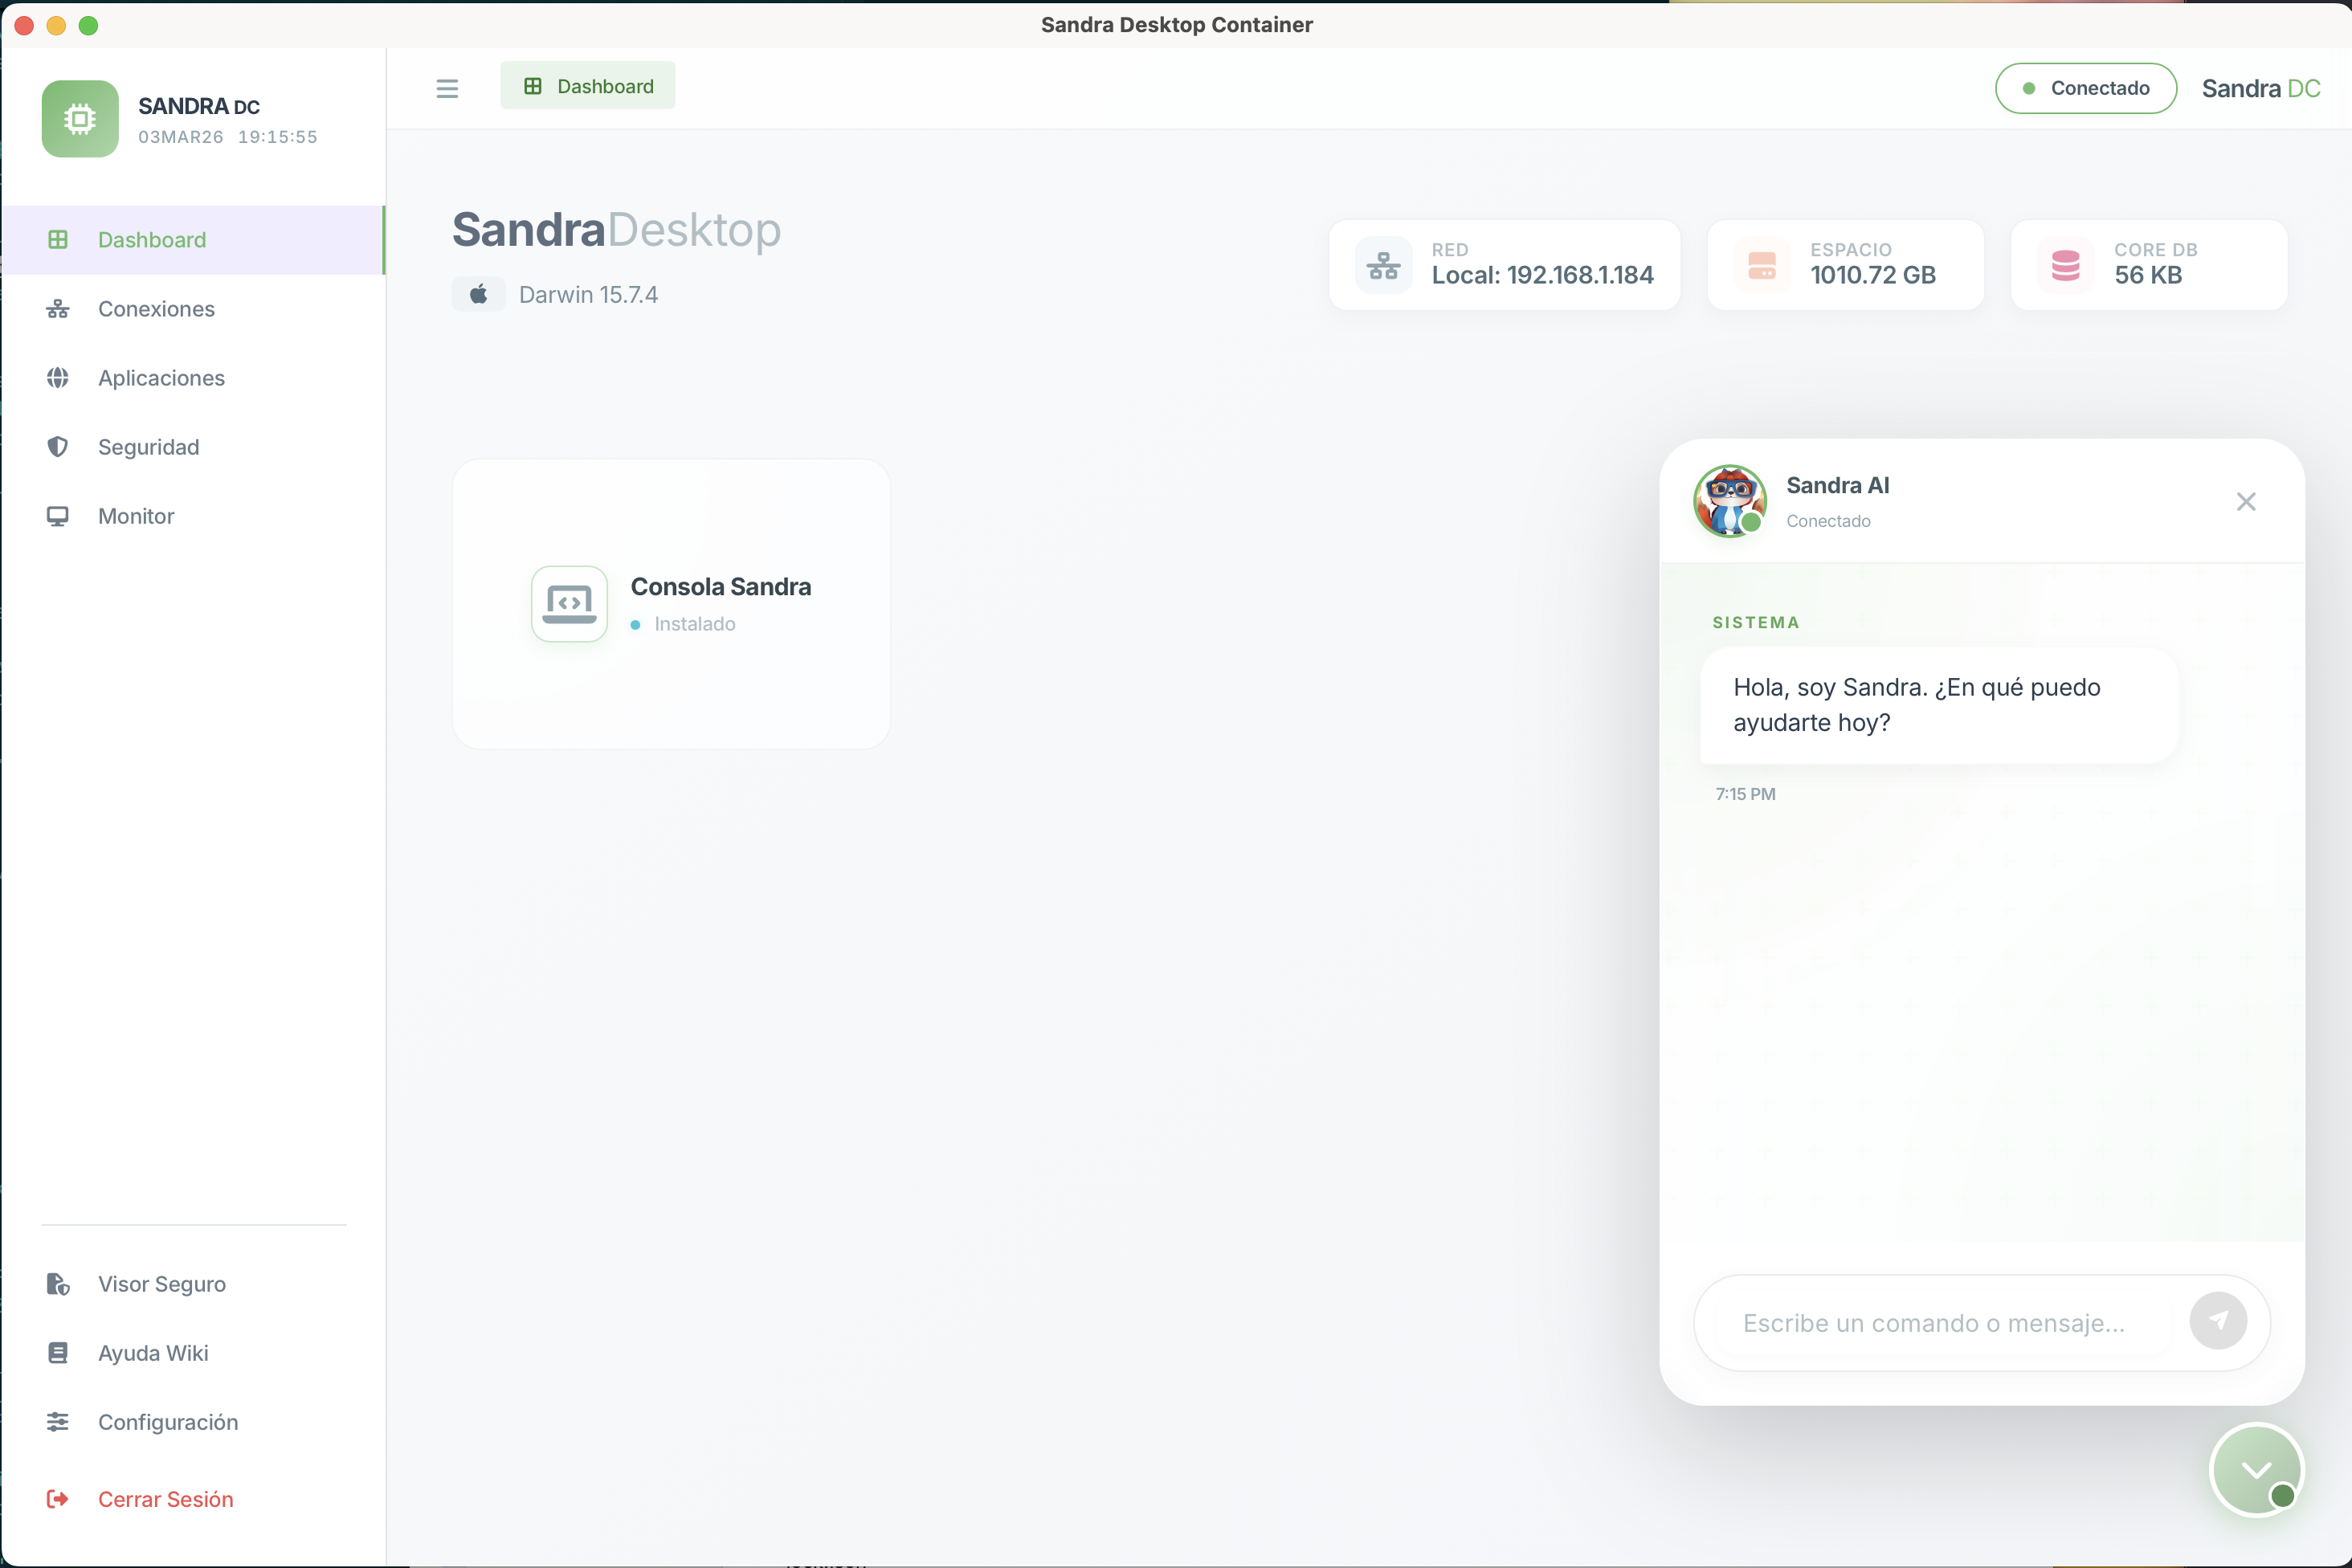
\includegraphics[width=0.95\textwidth]{anexos/4 principal.png}
\caption{Dashboard principal de Sandra Desktop Container}
\label{fig:dashboard}
\end{figure}

\subsection{Panel de Metricas del Sistema}

El dashboard presenta tres metricas fundamentales organizadas en tarjetas visuales:

\begin{table}[H]
\centering
\begin{tabular}{p{4cm}p{3cm}p{8cm}}
\toprule
\textbf{Icono FA} & \textbf{Metrica} & \textbf{Descripcion} \\
\midrule
\texttt{fa-network-wired} & RED & Estado de la conexion local, latencia y throughput \\
\midrule
\texttt{fa-hdd} & ESPACIO & Capacidad disponible en disco para contenedores \\
\midrule
\texttt{fa-database} & CORE DB & Base de datos SQLite interna cifrada \\
\bottomrule
\end{tabular}
\caption{Metricas principales del Dashboard}
\label{tab:metricas-dashboard}
\end{table}

\subsection{Interpretacion de las Metricas}

\subsubsection{Estado de RED}

La metrica de red muestra:
\begin{itemize}[leftmargin=*]
    \item Estado de conexion: Activa/Inactiva
    \item Interfaces detectadas: Ethernet, WiFi
    \item Latencia: Tiempo de respuesta en ms
    \item Throughput: Velocidad de transferencia
\end{itemize}

\begin{quote}
\textbf{Indicadores de Estado:}
\begin{itemize}
    \item \textbf{Verde}: Conexion estable y optima
    \item \textbf{Ambar}: Conexion lenta o inestable
    \item \textbf{Rojo}: Sin conexion o error
\end{itemize}
\end{quote}

\subsubsection{Espacio de Almacenamiento}

El espacio disponible se calcula considerando:
\begin{itemize}[leftmargin=*]
    \item Contenedores activos
    \item Datos temporales
    \item Logs de auditoria
    \item Cache de aplicaciones
\end{itemize}

\begin{quote}
\textbf{Advertencia:} Cuando el espacio desciende por debajo del 20 por ciento, SDC mostrara alerta.
\end{quote}

\section{Asistente Sandra AI}
\label{sec:sandra-ai}

\sandraai{} es una consola de inteligencia artificial ubicada en la esquina inferior derecha del dashboard.

\subsection{Activacion del Asistente}

Para iniciar una conversacion:
\begin{enumerate}[leftmargin=*]
    \item Hacer clic en el icono (clase FA: \texttt{fa-robot}) en la esquina inferior derecha
    \item Escribir la consulta en el campo de texto
    \item Presionar Enter
\end{enumerate}

\subsection{Tipos de Interaccion}

Sandra AI procesa tres categorias de consultas:

\begin{table}[H]
\centering
\begin{tabular}{p{4cm}p{4cm}p{6cm}}
\toprule
\textbf{Categoria} & \textbf{Ejemplo} & \textbf{Respuesta} \\
\midrule
Consultas Tecnicas & Que es una ruta proxy? & Explicacion conceptual \\
\midrule
Comandos Operativos & Crear nueva conexion & Asistente de configuracion \\
\midrule
Diagnostico & Por que no puedo conectarme? & Analisis de logs \\
\bottomrule
\end{tabular}
\caption{Tipos de interaccion con Sandra AI}
\label{tab:tipos-ai}
\end{table}

\subsection{Comandos Predefinidos}

\begin{lstlisting}[language=bash, caption={Comandos de Sandra AI}]
# Gestionar conexiones
- "nueva conexion"
- "listar conexiones"
- "eliminar conexion [nombre]"

# Gestionar aplicaciones
- "nueva aplicacion"
- "abrir aplicacion [nombre]"

# Informacion del sistema
- "estado del sistema"
- "espacio disponible"
- "logs de auditoria"
\end{lstlisting}

\section{Navegacion Principal}
\label{sec:navegacion}

Modulos de la barra lateral:

\begin{table}[H]
\centering
\begin{tabular}{p{3.5cm}p{10cm}}
\toprule
\textbf{Modulo (Icono FA)} & \textbf{Descripcion} \\
\midrule
\texttt{fa-th-large} Dashboard & Panel principal con metricas \\
\texttt{fa-code} Aplicaciones & Micro-aplicaciones desplegadas \\
\texttt{fa-plug} Conexiones & Servidores remotos \\
\texttt{fa-shield-alt} Seguridad & Politicas y auditoria \\
\texttt{fa-eye} Visor & Documentos seguros \\
\texttt{fa-cog} Configuracion & Preferencias \\
\bottomrule
\end{tabular}
\caption{Modulos de navegacion de SDC}
\label{tab:modulos-navegacion}
\end{table}

\subsection{Accesos Directos}

\begin{itemize}[leftmargin=*]
    \item \texttt{fa-plus} Nueva Conexion
    \item \texttt{fa-plus} Nueva Aplicacion
    \item \texttt{fa-sync} Sincronizar
    \item \texttt{fa-history} Auditoria
\end{itemize}

\section{Personalizacion del Dashboard}

\subsection{Temas de Color}

\begin{itemize}[leftmargin=*]
    \item \textbf{Tema Claro}: Paleta Sandra Teal Soft (default)
    \item \textbf{Tema Oscuro}: Optimizado para uso nocturno
    \item \textbf{Tema Alto Contraste}: Accesibilidad
\end{itemize}
